\chapter{Background}
\label{chap:background}

\section{Basics of Fully Homomorphic Encryption}
\gls{he} makes it possible to operate on data without knowing it.
One can distinguish three flavors of it, Partial-, Semi- and \gls{fhe}.

% Fully Homomorphic Encryption (FHE):
\begin{itemize}
  \item Brakerski/Fan-Vercauteren (BFV) scheme for integer arithmetic
  \item Brakerski-Gentry-Vaikuntanathan (BGV) scheme for integer arithmetic
  \item Cheon-Kim-Kim-Song (CKKS) scheme for real-number arithmetic
  \item Ducas-Micciancio (FHEW) and Chillotti-Gama-Georgieva-Izabachene (TFHE) schemes for Boolean circuit evaluation
\end{itemize}

\subsection{Packing}
FFT in CKKS!
Polynom -> Vektor mit einer FFT
Vektor -> Polynom mit einer IFFT

\subsection{HE using RSA}
With unpadded RSA, some arithmetic can be performed on the ciphertext - looking at the encrypted ciphertext $\mathcal{E}(m_1) = (m_1)^r \mod n$ of the message $m_1$ and $m_2$ respectively, the following holds:
\begin{align}
  \mathcal{E}(m_1) \cdot \mathcal{E}(m_2)
   & = (m_1)^r (m_2)^r \mod n     \\
   & = (m_1 m_2)^r \mod n         \\
   & = \mathcal{E}(m_1 \cdot m_2)
\end{align}

The encryption therefore partially fulfills the properties of ring homomorphism, which in general is defined as follows:

\begin{definition}{Ring Homomorphism}{ring-homomorphism} ~
  Given two rings $(R, +, \cdot)$ and $(S, \oplus, \otimes)$, we call a mapping $\varphi: R \rightarrow S$ a ring homomorphism when it satisfies the following conditions:
  $$\forall a, b \in R: \varphi(a + b) = \varphi(a) \oplus \varphi(b) \wedge \varphi(a \cdot b) = \varphi(a) \otimes \varphi(b)$$
\end{definition}

\subsection{Learning with Errors (LWE)}

\subsection{Ring-LWE}
Learning with Errors on Rings (RLWE)

how to get from LWE to RLWE

\subsection{The BFV scheme}
\subsection{The CKKS scheme}
The CKKS scheme allows us to perform approximate arithmetic on floating point numbers.

\section{Machine Learning}
As Shafi Goldwasser puts it, 'Machine Learning is somewhere in the intersection of Artificial Intelligence, Statistics and Theoretical Computer Science' \cite{goldwasserTalk2018}.

\begin{figure}
  \centering
  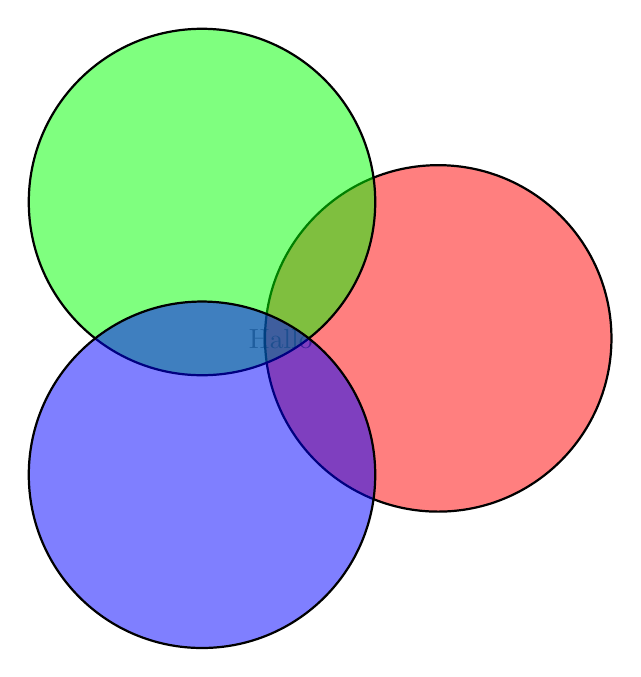
\begin{tikzpicture}[thick]
    % \node[draw=red, fill=red!30, fill opacity=0.5, minimum size=2cm, circle] (ref1);
    \filldraw[fill=red,fill opacity=0.5] (0:2cm) node [midway, black] {Hallo} circle (22mm);
    \filldraw[fill=green,fill opacity=0.5] (120:2cm) circle (22mm);
    \filldraw[fill=blue,fill opacity=0.5] (-120:2cm) circle (22mm);
  \end{tikzpicture}
  \caption{Ah yes the caption}
\end{figure}

\subsection{Linear Regression?}
\subsection{Gradient Descent?}
\subsection{The Backpropagation Algorithm}
\subsection{Multi-Layered Neural Networks}
Matrix -> Activation Function
\begin{itemize}
  \item Matrix Multiplication (Dense Layer)
  \item Convolutional Layer
  \item Sigmoid Activation
  \item Max Pooling
\end{itemize}

\section{Post-Quantum Security}

\section{Demo}
In this chapter, we provide some usage examples for
glossaries and acronym lists with \texttt{glossaries} (\autoref{sec:gloss}),
bibliography and citations with \texttt{biblatex} (\autoref{sec:bib}), and more.

\begin{figure}[H]
  \centering
  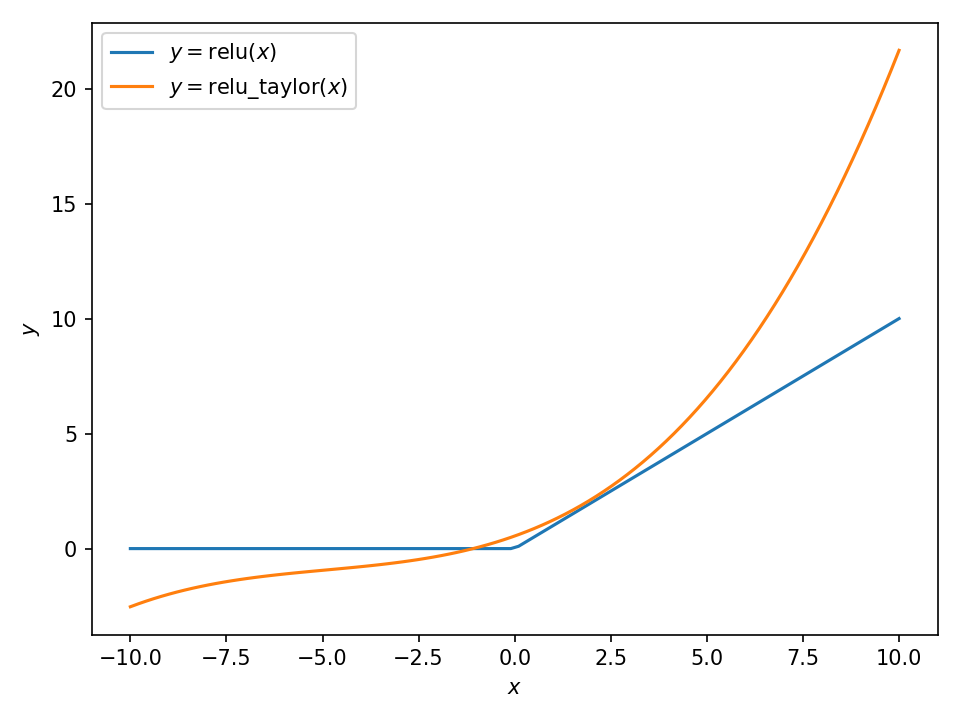
\includegraphics[width=0.8\linewidth]{figures/taylor-relu.png}
  \caption{Comparison of the Relu activation function vs. its Taylor expansion}
\end{figure}

\section{Notation and Acronyms}
\label{sec:gloss}
Symbols and acronyms are defined in the preamble, after loading the \texttt{glossaries} package, and used as follows.

\lipsum

In this chapter, we introduce the necessary background on the \gls{aes}.
We denote binary exclusive-or by \gls{xor}.

\section{Citations}

\lipsum

\label{sec:bib}
This is an example of how to specify and cite
a book \cite{AESbook},
a journal article \cite{bstjShannon49}.
\Gls{aes} is a block cipher defined by \textcite{AESbook}.
